% !TEX root = thesis.tex
\documentclass[thesis]{subfiles}

\begin{document}
	\chapter{Conditional Connectivity}\label{conditionalnetworks}
	%\chapter{Conditional Computation in Deep Neural Networks}
	\begin{chapquote}{David Rumelhart, \textit{in personal communication with \citeauthor{hanson1989comparing}, 1987}}
		``\ldots the simplest most robust network which accounts for a data set will, on average, lead to the best generalization to the population from which the training set has been drawn''
	\end{chapquote}
	
	The ideal discriminative model desired for most tasks would have all the advantages of both neural networks and decision forests, and none of the weaknesses. It would have good generalization with computational efficiency, lend itself to semantic understanding and yet have sufficient functional complexity to solve complex problems. 
	
	In this chapter we intend to explore the continuum of discriminative models that exist between decision forests and neural networks\index{neural network}, to try to find such a balance. We will explore the theory and applications behind such models, with a focus on contemporary problems such as object class recognition, \ie the ImageNet \gls{ilsvrc} challenge which has been the focus of much of the recent work on deep learning.
	
	\section{On Methods of Discriminative Classification}
	Two methods of discriminative classification, \emph{Neural Networks} and \emph{Decision Forests}, have recently dominated the field of Computer Vision. Deep neural networks\index{neural network} have even replaced the research in local features (\eg \gls{sift}), providing end-to-end learning from pixels to output~\citep{yi2016lift}. Much work has been done on improving both methods and exploring their applications --- with academic and even commercial success. For example, decision forests are used to find the body pose of a person with the Kinect~\citep{conf/cvpr/ShottonFCSFMKB11} used in game consoles. Deep \glspl{cnn}\index{CNN} on the other hand have recently surpassed human accuracy on what was considered one of the most challenging outstanding problems in computer vision, object class recognition~\citep{He2015b}, and are already finding their ways into applications such as Google Photos\footnote{\href{http://photos.google.com}{http://photos.google.com}}. However, the important fact that these two methods are related often seems to be all but forgotten. \citet{Sethi1990} showed that any decision tree can be represented as a neural network\index{neural network} with one hidden layer, however the converse does not necessarily hold true.
	
	Despite this fundamental relationship, decision forests and neural networks\index{neural network} have such distinct and mutually exclusive strengths and weaknesses that it is not surprising that they are themselves usually considered to be distinct. Decision forests require vast amounts of labelled data, proportional to the number of classes and tree depth, since samples are ``diluted'' down the tree, while, with appropriate regularization, neural networks\index{neural network} can be trained with far more parameters than actual samples. At test time, neural networks\index{neural network} are opaque giving little understanding, while decision forests are more intuitive --- each node having an explicit decision on the input data and even describe per-class statistics. The routing of decision forests makes it easy to distribute computation, while the high connectivity of neural networks\index{neural network} makes model parallelism difficult and inefficient. Decision forests are extremely fast at test time due to sample routing, only a small part of a tree need be computed, \ie conditional computation. Neural networks\index{neural network} must, on the other hand, computation the response at every node, even if many of these responses are approximately zero or not useful to the final output.
	
	\section{Generalizing \Glsfmtplural{dnn} and Decision Trees}
	Here we explore the continuum of models between decision forests, with the objective of reducing the connectivity of deep neural networks\index{neural network} trained with backpropagation\index{backpropagation}, specifically \glspl{cnn}, while retaining some of the efficiency and understanding which arise from the conditional computation in decision forests.
	
	Towards this objective, we generalize neural networks\index{neural network} and decision trees intuitively by using a new graphical notation for representing both. This notation isolates the differences between the two models, such that we can represent a hybrid model, \ie a \emph{Conditional Network}, compactly\footnote{This notation itself was created by Dr.\ Antonio Criminisi, and is not a contribution of this dissertation. Some figures are used with the permission of Dr.\ Antonio Criminisi/Microsoft Research.}.
	
	\section{A New Graphical Notation}
	The proposals we will make require a re-interpretation of existing classification models, that is neural networks\index{neural network} and decision trees, but standard graphical diagrams for both of these models hides the implicit functional similarities on which we will build our models, and are instead connection-centric --- focused on showing the connectivity of the models rather than the underlying data transformations. As such, before we are able to explain the concept of a conditional network, a new graphical language is proposed.
	
	\subsection{Neural Networks}
	\begin{figure}[tbp] 
		\centering
		\begin{subfigure}[b]{0.45\textwidth}
			\centering
			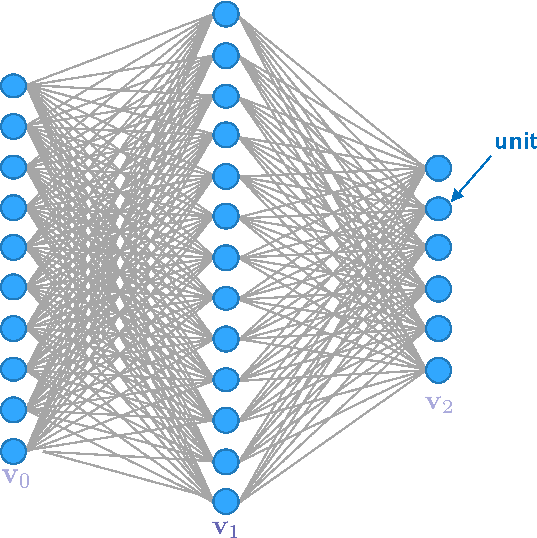
\includegraphics[width=\textwidth]{fullyconnected}
			\caption{Standard diagram of a neural network with one hidden layer.}\label{fig:oldnotation}
		\end{subfigure}
		~
		\begin{subfigure}[b]{0.45\textwidth}
			\centering
			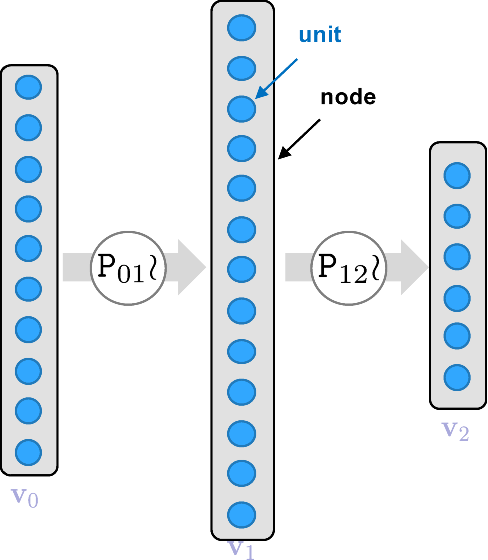
\includegraphics[width=0.9\textwidth]{newnotation}
			\caption{New notation showing transformation between layers explicitly.}\label{fig:newnotation}
		\end{subfigure}
		\caption[New graphical notation for neural networks]{\textbf{The proposed compact graphical notation for neural networks.} Non-linear transformations in a standard neural network\index{neural network} with one hidden layer are indicated by the projection matrix $\mat P$ between the two layers, followed by a generic non-linearity, represented with the symbol $\wr$. \copyright Antonio Criminisi, used with permission.}\label{fig:newGraphLanguage}
	\end{figure}
	
	The standard depiction of a neural network\index{neural network} with one hidden layer is shown in \cref{fig:oldnotation}, where each of the layers is fully-connected, and these connecting weights are illustrated as lines between the neurons\index{neuron} represented as circles. While this image illustrates the connectivity of the model, it assumes the function of the neurons\index{neuron} themselves to be known or otherwise described. In \cref{fig:newnotation}\ we use a different notation to show both connectivity and function of each layer, with the assumption that all nodes on a particular layer have the same function.
	
	In this simple example of a fully-connected neural network\index{neural network}, between layers $i$ and $j$, every node outputs the non-linear transformation, $\vec v_j = \sigma(\mat P \vec v_i)$, a composition of the non-linear function $\sigma$ (\eg a \gls{relu} or sigmoid) and the projection of the input units with a projection matrix $\mat P$, which includes the bias term in homogeneous coordinates. We denote this operation explicitly as $\mat P_{ij} \wr$, where $\mat P_{ij}$ is the projection matrix and $\wr$ represents a non-linearity. In short $\mat P_{ij} \wr$ denotes the standard neural net layer's non-linear transformation $\vec v_j = \sigma(\mat P \vec v_i)$. 
	
	\Glspl{cnn} typically include layers with pooling operations (\eg \gls{gap}), or local response normalization. Any of these operations may also be represented by the function $\sigma$.
	
	\subsection{Decision Trees and Random Forests}
	
	\begin{figure}[tbp] 
		\centering
		\begin{subfigure}[b]{\textwidth}
			\centering
			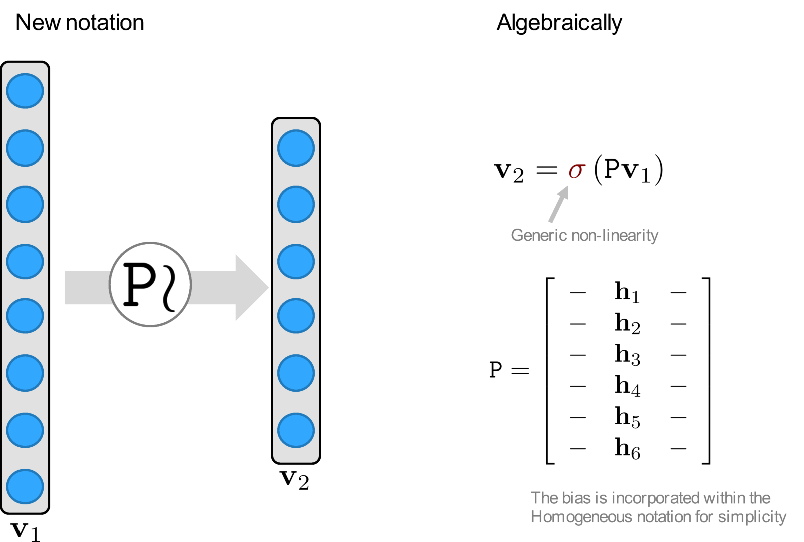
\includegraphics[width=0.7\textwidth]{projectionnotation}
			\caption{Generic projection with non-linearity, typically found in neural networks.}\label{fig:projectionnotation}
		\end{subfigure}
		~
		\begin{subfigure}[b]{\textwidth}
			\centering
			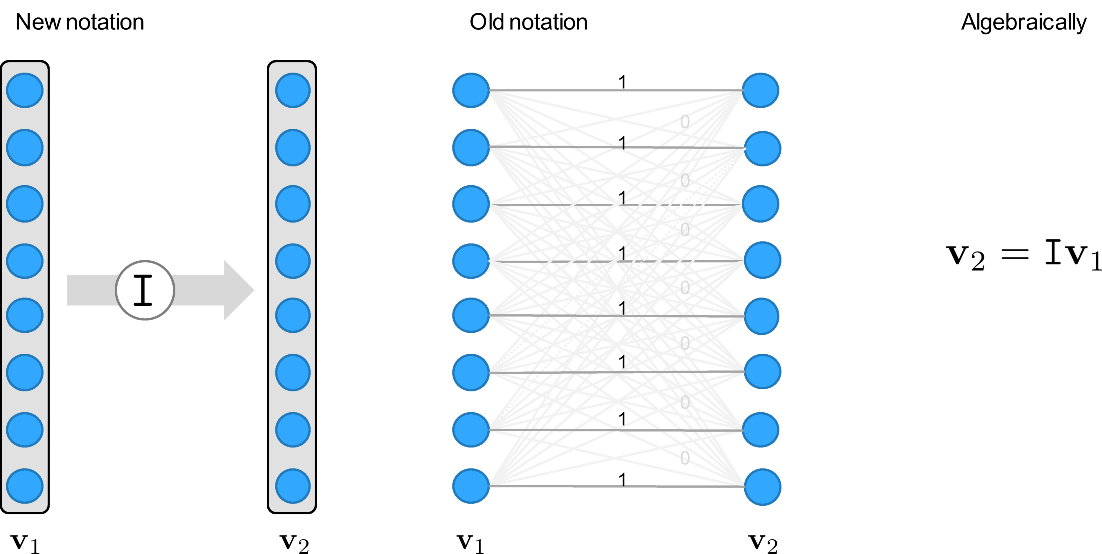
\includegraphics[width=0.9\textwidth]{identitynotation}
			\caption{Identity projection with identity function, typically found in decision trees.}\label{fig:identitynotation}
		\end{subfigure}
		~
		\begin{subfigure}[b]{\textwidth}
			\centering
			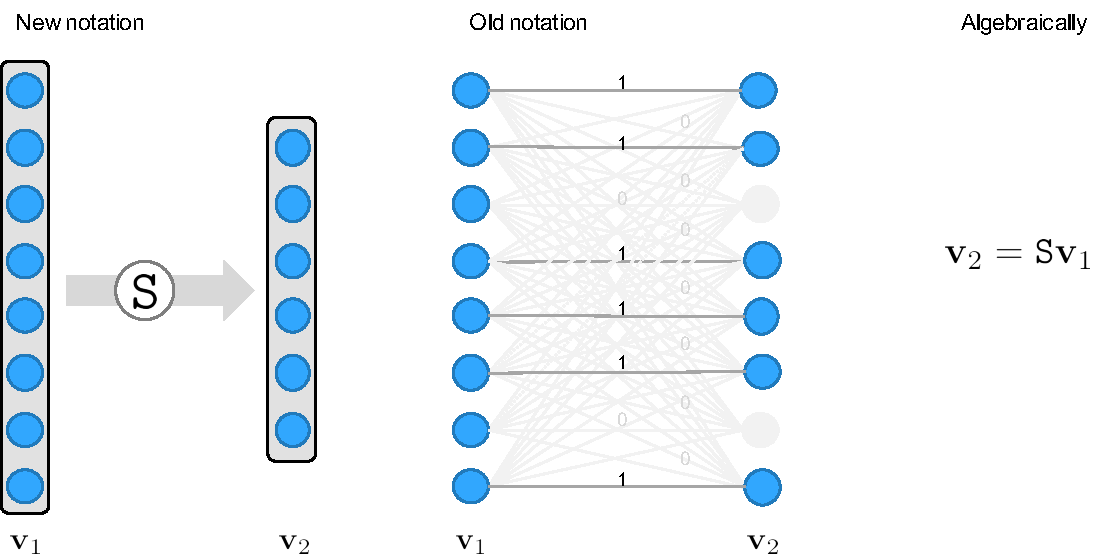
\includegraphics[width=0.9\textwidth]{selectionnotation}
			\caption{Selection projection, found in random forests.}\label{fig:selectionnotation}
		\end{subfigure}
		\caption[Various projection matrices in conditional networks]{\textbf{The proposed compact graphical notation for various types of projection in a conditional network.} \copyright Antonio Criminisi, used with permission.}\label{fig:projections}
	\end{figure}
	
	This graphical language may also represent decision trees, also typically depicted in a connection-centric graphical diagram as shown in \cref{fig:oldtreenotation}. Decision trees typically copy, or reference, samples from the root of the tree down to the leaf (or leaves) without transformation. This is notably in contrast with representation learning approaches, such as neural networks\index{neural network}, which try to learn optimal data transformations during training with a full projection matrix, as illustrated in \cref{fig:projectionnotation}. There have, however, been attempts to incorporate representation learning within decision forests~\citep{montillo2011entangled,BuloKontsch2014}. The copying of the sample may also be considered as a special case of the transformation $\vec v_j = \sigma(\mat P \vec v_i)$, where the projection is the identity matrix $\mat P_{ij} = \mat I$, and the function $\sigma$ is the identity function $\sigma(\vec v_i) = \vec v_i$. As such, we use the identity $\mat I$ in our graphical language to denote the routing between each tree level. This is explained graphically in \cref{fig:identitynotation}.
	
	Random forests consist of a number of decision trees, each of which is applied to a restricted number of the input feature dimensionality. It may not be immediately obvious how this is represented in our new graphical language, but in fact a simple extension of the above theme represents selection --- \ie an identity matrix of reduced rank, as illustrated in \cref{fig:selectionnotation}.
	
	\subsection{Explicit Routing}
	\begin{figure}[htbp!] 
		\centering
		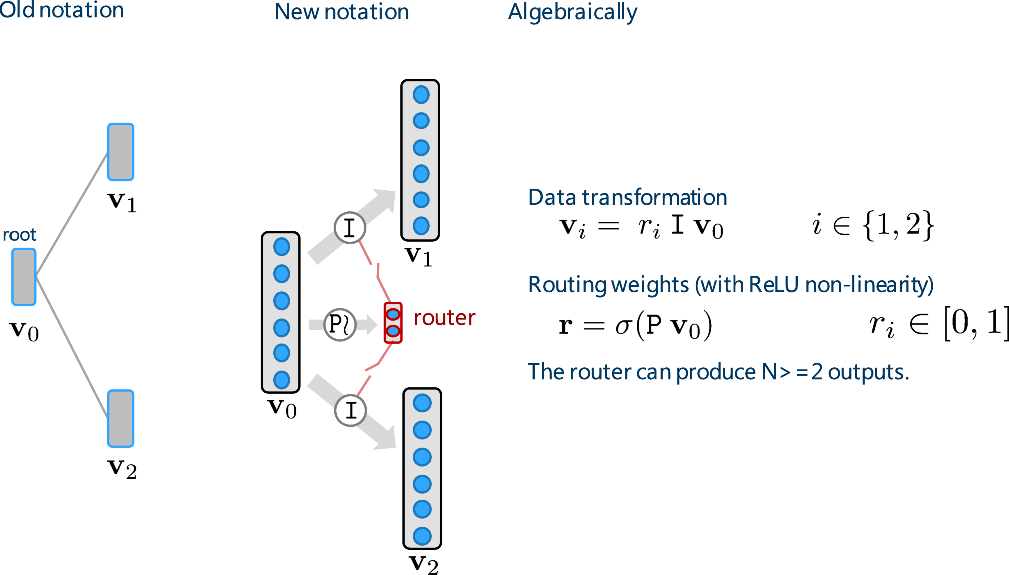
\includegraphics[width=0.95\textwidth]{treenotation}
		\caption[Proposed graphical notation for a decision stump]{\textbf{The proposed compact graphical notation for a ``decision stump''.}}\label{fig:treeNotation}
	\end{figure}
	
	\begin{figure}[tbp] 
		\centering
		\begin{subfigure}[b]{0.4\textwidth}
			\centering
			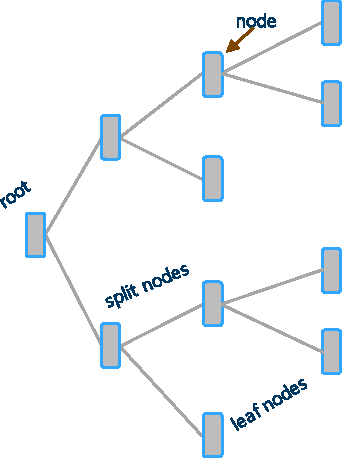
\includegraphics[width=0.95\textwidth]{oldtreenotation}
			\caption{Standard diagram of a decision tree.}\label{fig:oldtreenotation}
		\end{subfigure}
		~
		\begin{subfigure}[b]{0.4\textwidth}
			\centering
			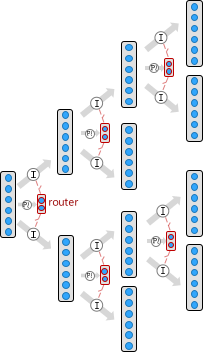
\includegraphics[width=0.8\textwidth]{newtreenotation}
			\caption{New explicit graphical notation.}\label{fig:newtreenotation}
		\end{subfigure}
		\caption[Proposed compact graphical notation for a decision tree]{\textbf{The proposed compact graphical notation for a full decision tree.} \copyright Antonio Criminisi, used with permission.}\label{fig:complexDecisionTree}
	\end{figure}
	
	We are still missing the method of conditional computation found in decision trees in our graphical language however, \ie how the decision is made to route each sample at a node. We must generalize two forms of routing found in decision trees, \emph{hard routing} where samples are only routed to one node in the next layer, and \emph{soft routing} where a weighted sample is potentially sent to every node of the next layer.
	
	We achieve this with the minor addition of a new set of nodes we call \emph{routers}. A router consists of $K$ weights for a $K$-ary node or tree, as shown in \cref{fig:treeNotation}. These router weights themselves are determined in a way more reminiscent of a neuron's\index{neuron} activation function, typically a non-linear transformation of the sample. Thus this is represented in the same graphical notation as the mapping between neural network\index{neural network} layers, \ie as $\mat P_{ij} \wr$. \Cref{fig:newtreenotation} shows the same tree as shown in \cref{fig:oldtreenotation}, notably with the routers highlighted in red. Typically a router will have a number of non-zero weights and perform soft routing, however if only one of the router weights is non-zero, the router effects hard routing.
	
	
	\begin{figure}[tbp] 
		\centering
		\begin{subfigure}[b]{0.45\textwidth}
			\centering
			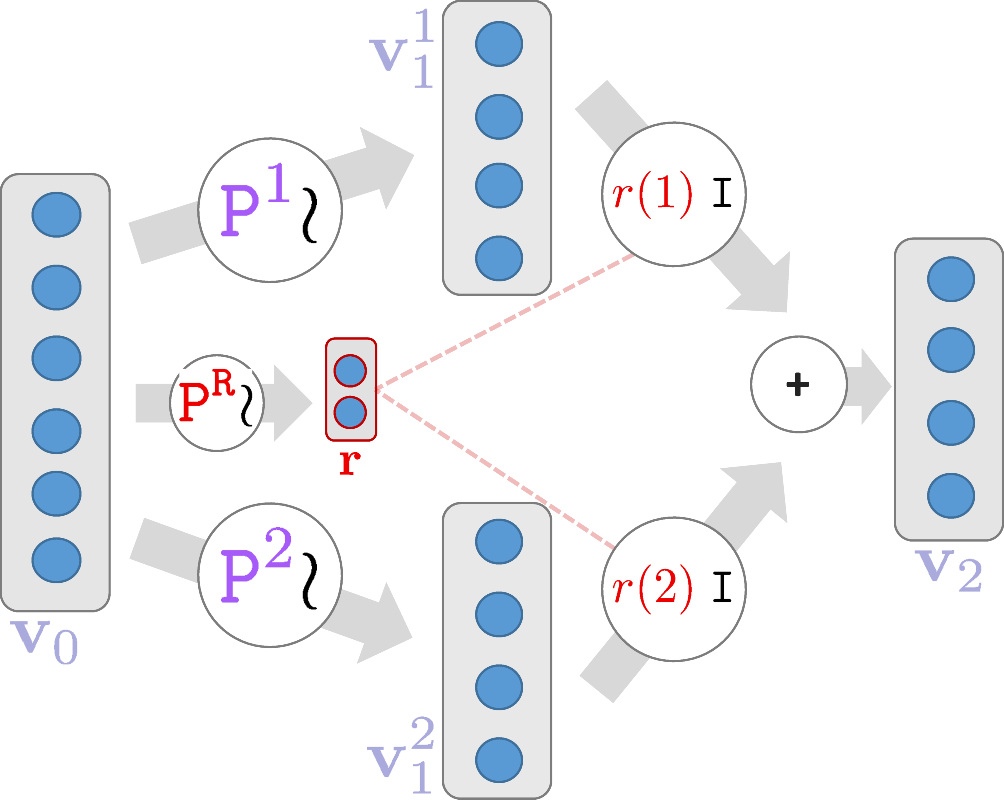
\includegraphics[width=0.95\textwidth]{explicit}
			\caption{Explicitly routed network.}\label{fig:explicitRouter}
		\end{subfigure}
		~
		\begin{subfigure}[b]{0.45\textwidth}
			\centering
			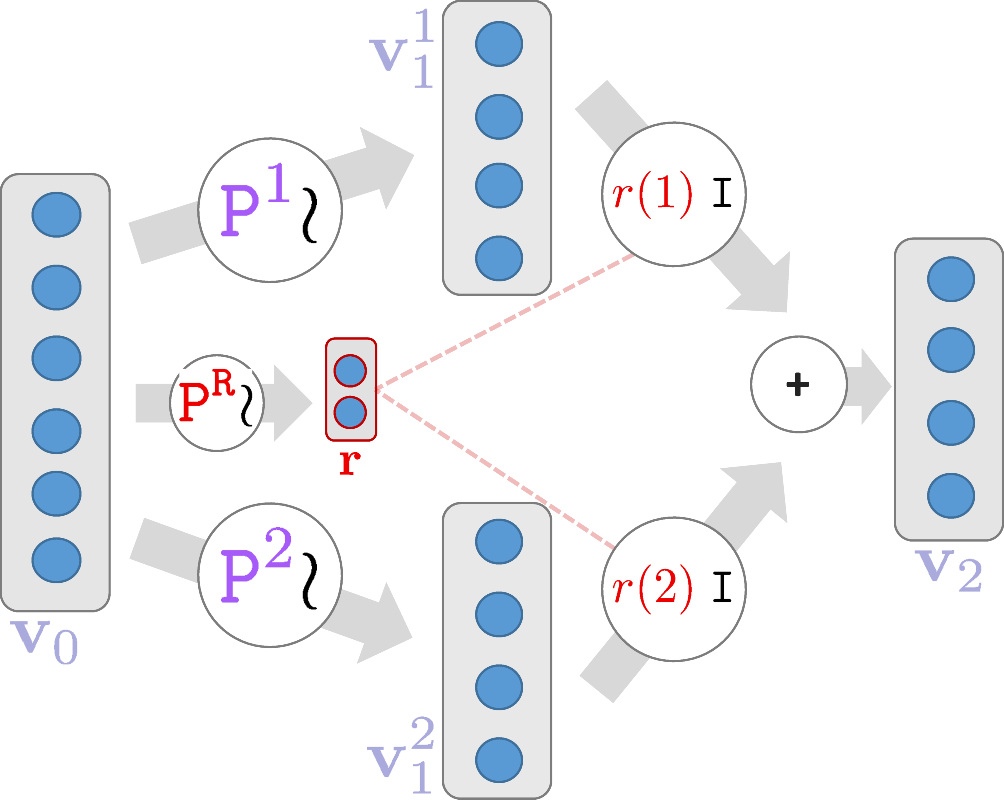
\includegraphics[width=0.95\textwidth]{explicit}
			\caption{Implcitly routed network.}\label{fig:implicitRouter}
		\end{subfigure}
		\caption[Explicit \vs implicitly routed networks]{\textbf{Explicit \vs implicitly routed networks.} \copyright Antonio Criminisi, used with permission.}\label{fig:routerConnections}
	\end{figure}
	
	\subsection{Implicit Routing}
	It is in fact possible for networks to learn a conditional routing of data without an explicit router. We call this form of conditional routing \emph{\gls{implicitrouting}\index{implicit routing|textbf}} \vs \emph{\gls{explicitrouting}\index{explicit routing|textbf}}, where a router is used. 
	
	In an explicitly routed network, the routes are trained by combining the routes before the training loss. For example, in \cref{fig:explicitRouter} the input to layer $v_2$, $y_1$, is a linear combination of the routes weighted by the router weights, represented by $\circleplus$ operator,
	\begin{equation}
	y_1 = \left\{y_1^j\right\} \forall j\circleplus \vec r = \sum_j r_j \sigma\left(P^j \vec v_1^j \right).
	\end{equation}
	
	For an implicitly routed network instead a (non-weighted) linear combination is followed by a single fully-connected layer, \ie inner product and \gls{relu}, \ie for \cref{fig:implicitRouter}, the output of $\vec v_2$, is simply,
	\begin{equation}
	y_1 = \max \left(0, ~\sum_j v_1^j \sigma(P^j \vec v_0) \right).
	\end{equation}
	
	\subsection{Conditional Networks}
	The generalization, a conditional network, mixes elements of both of these models. Conditional networks may perform arbitrary projections of samples, and use arbitrary non-linear functions. Conditional networks may route samples with a soft or hard router in some or all of the layers, they may select some of all of the input feature space. 
	
	\section[Results]{Results\protect\footnote{Note, two interesting experiments are omitted here because they are primarily the work of my co-authors, Antonio Criminisi and Duncan Robertson. I refer interested readers to the technical report for completeness: \citet{Ioannou2015}.}}
	\subsection{\Glsfmttext{ilsvrc}}
	We first validate the use of conditional networks for image classification on the \gls{ilsvrc} dataset~\citep{ILSVRC2015}, a large dataset consisting of 1.2M training images for 1000 classes, and 50,000 validation images.
	
	As discussed in \cref{alexnetfiltergroups}, AlexNet uses two filter groups\index{filter groups} throughout most of the layers of the model in order to split computation across two \gls{gpu}s. The authors observed that the filters on each \gls{gpu} appeared to specialize to learn fundamentally different features regardless of initialization~\citep{Krizhevsky2012}. This interesting observation has mostly been ignored in subsequent networks where \gls{gpu} memory has increased enought that such a split of the network is not required, but the original observation is a fundamental motivation of our work.
	
	We based our experiments on the VGG network~\citep{Simonyan2014verydeep} on which the current state-of-the-art models are also based~\citep{He2015b}. Specifically, we focus on the \gls{vgg}-11 model as it is deep (11 layers) and relatively memory efficient (trains with Caffe~\citep{Jia2014} on a single Nvidia K40 \gls{gpu}). It notably does not have any filter group\index{filter groups}ing, as found in AlexNet, or low-dimensional embeddings, as found in \gls{nin}. It therefore suffers from an explosion in the number of filters required at each layer, and represents the ideal network on which to demonstrate the efficiency savings brought about by these simple modifications.
	
	\subsubsection{Global Max-Pooling to Reduce Model Size}
	We found that \gls{gmp}, like \gls{gap} (as used by \citet{Lin2013NiN,Szegedy2014going}), after the last convolutional layer is effective in reducing model parameters while maintaining, if not improving, accuracy. This suggests that preserving spatial information after the convolutional layers may not be as important as previously thought. 
	We trained a new network (`\gls{vgg}-11-GMP') with such pooling, and achieved lower top-5 error than the baseline \gls{vgg}-11 
	network (13.3\% \vs 13.8\%), with a decrease in the number of parameters of over 72\% (see \cref{fig:VggPerLayerCost}).
	
	\subsubsection{Designing an Efficient Conditional Architecture}
	Starting from the already improved, non-routed \gls{vgg}-11-GMP architecture, we designed the conditional network in \cref{fig:Imagenet_CondNet}.
	% figure 
	\begin{figure}[tbp]
		\centering
		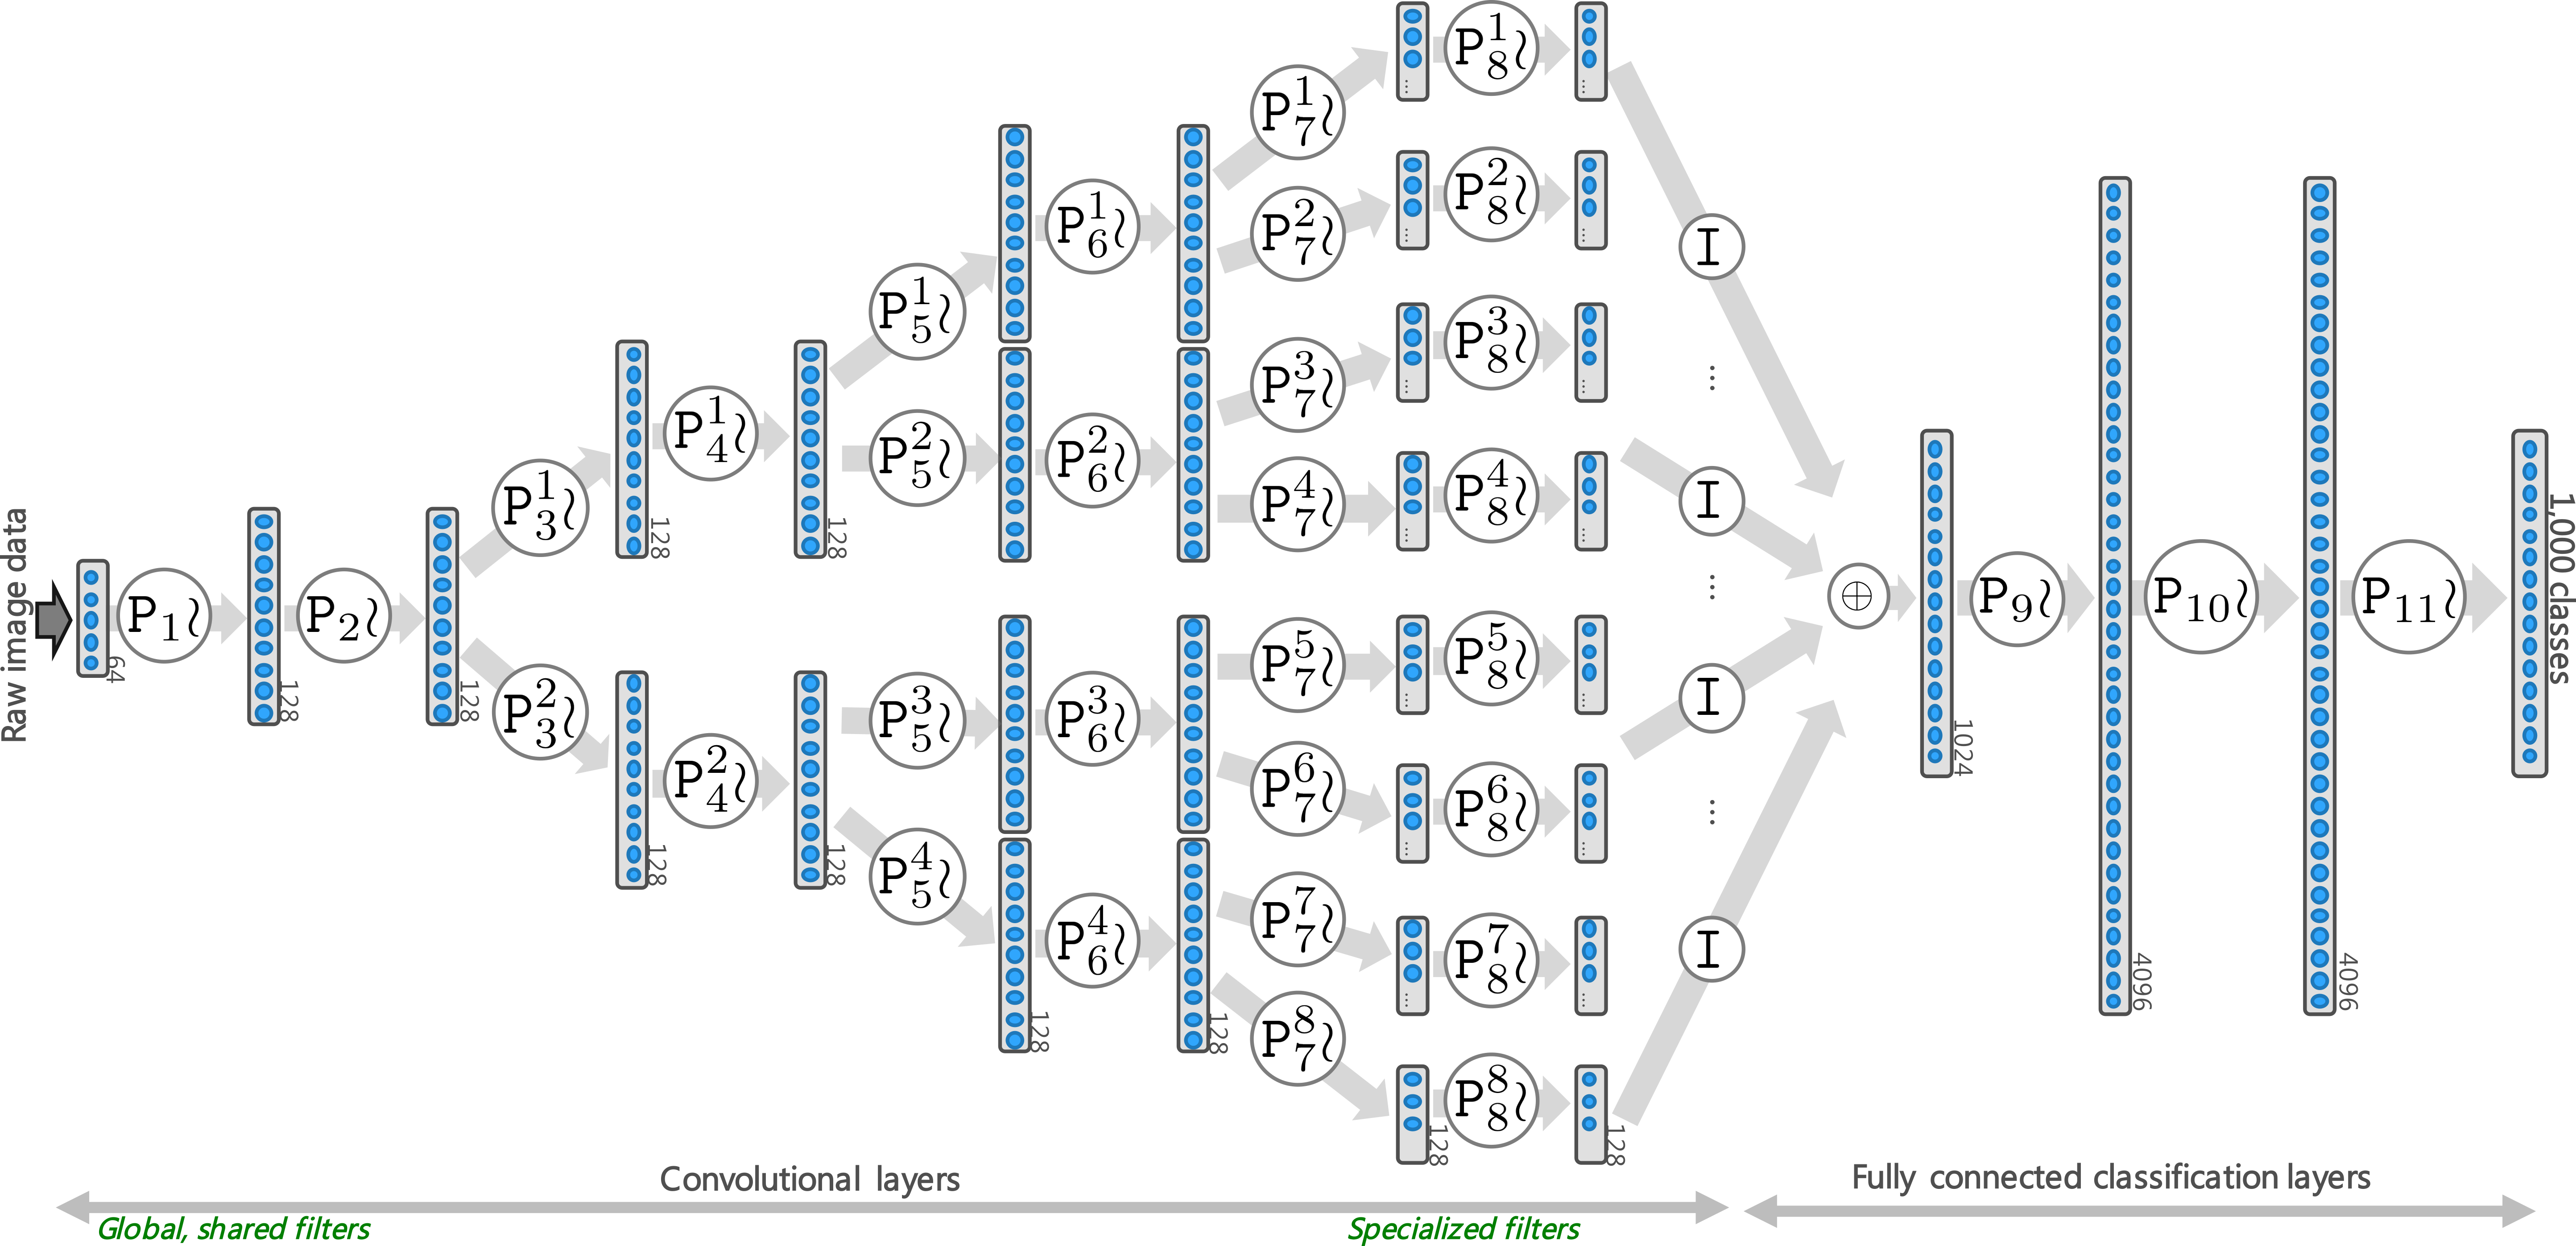
\includegraphics[width=\linewidth]{resultsImagenet_conditionalNetwork}
		\caption[Conditional network used with ILSVRC experiments]{\textbf{Conditional network used with Imagenet experiments.} The network employs implicit data routing in the (expensive) convolutional layers to yield higher computational efficiency than the corresponding, non-routed \glsfmtplural{dnn}\index{DNN}.}\label{fig:Imagenet_CondNet}
	\end{figure}
	%
	Since most of the computational cost in \gls{vgg}-11-GMP is in the convolutional layers, our conditional variant 
	introduces a DAG-like routed structure to split the filters in the convolutional section.
	The assumption here is that each filter should only need to be applied to a small number of channels in the input \gls{featuremap}\index{featuremap}.
	
	Data routing is implemented via `filter groups\index{filter groups}', as originally used in~\citep{Krizhevsky2012}. 
	Thus, at each level $\textrm{conv}\_n\_\{1,2\}, n=3\ldots 5$, the convolutional filters of \gls{vgg}-11-GMP are 
	divided into $2^{(n-2)}$ groups. Each group depends only on the results of exactly 128 previous filters. 
	The \glspl{featuremap}\index{feature map} of the last convolutional layer are concatenated together, and globally max-pooled
	before the fully-connected layers, which remain the same as those in \gls{vgg}-11-GMP.
	
	\subsubsection{Training}
	We trained our conditional network with the same hyperparameters as in~\citep{Simonyan2014verydeep}, 
	except for using the initialization strategy suggested of~\citep{He2015b}, and a learning schedule,
    \begin{equation}
        \gls{lr}_t = \gls{lr}_0(1+\gls{lr}_0\gls{weightdecay} \gls{t})^{-1},
    \end{equation}
	where $\gls{lr}_0,\gls{lr}_t$ and $\gls{weightdecay}$ are the initial learning rate, learning rate at iteration $\gls{t}$, and weight decay\index{weight decay} respectively~\citep{Bottou2012sgdtricks}.
	When the validation accuracy of the network levelled out, the learning rate was further decreased by a factor of 10, twice. 
	The conditional network took twice as many epochs to train than \gls{vgg}-11, however this equates to a comparable
	training time given its higher efficiency.

	\subsubsection{Accuracy \vs Efficiency}
	In order to compare different network architectures as fairly as possible, here we did not use any training
	augmentation aside from that supported by Caffe~\citep{Jia2014} (mirroring/random crops). Similarly we report test-time 
	accuracy based only on centre-cropped images, without potentially expensive data oversampling. 
	This reduces the overall accuracy (w.r.t.\ to state of the art), but constitutes a fairer test bed for teasing out the effects of different network architectures. This is because each architecture uses a different method of augmentation and has a different affect on the increase in inference time.
	Applying the same oversampling to all networks produced a nearly identical accuracy improvement in 
	all models, without changing their ranking.

	%%% Figure ---------------
	\begin{figure}[tbp]
		\centering
		\begin{subfigure}[b]{0.98\linewidth}
			\pgfplotstableread[col sep=comma,]{condnetdata/condnetdata-stride1.csv}\datatablea
			\pgfplotstableread[col sep=comma,]{condnetdata/condnetdata-stride2.csv}\datatableb
			\pgfplotstableread[col sep=comma,]{condnetdata/condnetdata-stride4.csv}\datatablec
			\pgfplotsset{major grid style={dotted,red}}
			
			\centering
			\begin{tikzpicture}
			%\tikzstyle{every node}=[font=\footnotesize]
			\begin{axis}[
				width=0.95\linewidth,
				height=0.4\textheight,
				axis x line=bottom,
				ylabel=Top-5 Error (Centre-Crop),
				xlabel=\gls{flops} (Multiply-Add),
				axis lines=left,
				enlarge x limits=0.1,
				enlarge y limits=0.05,
				grid=major,
				%xmin=0,
				%ytick={0.002,0.004,...,1.0},
				%ymin=0.075,ymax=0.09,
				xticklabel style={
					/pgf/number format/fixed zerofill,
					/pgf/number format/precision=1
				},
				yticklabel={\pgfmathparse{\tick*1}\pgfmathprintnumber{\pgfmathresult}\%},style={
					/pgf/number format/fixed,
					/pgf/number format/precision=1
				},
				\setplotcyclecat{3},
				every axis plot/.append style={fill},
				legend style={at={(1,1.1)}, anchor=south east, column sep=0.2em, font=\footnotesize},
				legend columns=4,
			]
			\addplot+[mark=*,
				nodes near coords,
				only marks,
				point meta=explicit symbolic,
				every node near coord/.append style={xshift=0.01em, anchor=west, font=\footnotesize},
			] table[meta=Network Name,x=Multiply-Acc Ops,y expr = {\thisrow{Top-5 Error (centre crop)}*100},]{\datatablea};
			\addplot+[mark=square*,
				nodes near coords,
				only marks,
				point meta=explicit symbolic,
				every node near coord/.append style={xshift=0.01em, anchor=west, font=\footnotesize},
			] table[meta=Network Name,x=Multiply-Acc Ops,y expr = {\thisrow{Top-5 Error (centre crop)}*100},]{\datatableb};
			\addplot+[mark=diamond*,
				nodes near coords,
				only marks,
				point meta=explicit symbolic,
				every node near coord/.append style={xshift=0.01em, anchor=west, font=\footnotesize},
			] table[meta=Network Name,x=Multiply-Acc Ops,y expr = {\thisrow{Top-5 Error (centre crop)}*100},]{\datatablec};
			\legend{\texttt{conv1}/1, \texttt{conv1}/2, \texttt{conv1}/4}
			\end{axis}
			\end{tikzpicture}
			%\caption{\textbf{\glsfmttext{flops} (Multiply-Add) \vs Error.}}
			%\label{fig:nincifarmaconvonly}
		\end{subfigure}
		\vfill
		\begin{subfigure}[b]{0.98\linewidth}
			\pgfplotstableread[col sep=comma,]{condnetdata/condnetdata-stride1.csv}\datatablea
			\pgfplotstableread[col sep=comma,]{condnetdata/condnetdata-stride2.csv}\datatableb
			\pgfplotstableread[col sep=comma,]{condnetdata/condnetdata-stride4.csv}\datatablec
			\pgfplotsset{major grid style={dotted,red}}
			
			\centering
			\begin{tikzpicture}
			%\tikzstyle{every node}=[font=\footnotesize]
			\begin{axis}[
				width=0.95\linewidth,
				height=0.4\textheight,
				axis x line=bottom,
				ylabel=Top-5 Error (Centre-Crop),
				xlabel=Model Parameters,
				axis lines=left,
				enlarge x limits=0.1,
				enlarge y limits=0.05,
				grid=major,
				xmin=0,
				%ytick={0.002,0.004,...,1.0},
				%ymin=0.075,ymax=0.09,
				xticklabel style={
					/pgf/number format/fixed,
					/pgf/number format/precision=1
				},
				yticklabel={\pgfmathparse{\tick*1}\pgfmathprintnumber{\pgfmathresult}\%},style={
					/pgf/number format/fixed,
					/pgf/number format/precision=1
				},
				\setplotcyclecat{3},
				every axis plot/.append style={fill},
			]
			\addplot+[mark=*,
				nodes near coords,
				only marks,
				point meta=explicit symbolic,
				every node near coord/.append style={xshift=0.01em, anchor=west, font=\footnotesize},
			] table[meta=Network Name,x=Num Parameters,y expr = {\thisrow{Top-5 Error (centre crop)}*100},]{\datatablea};
			\addplot+[mark=square*,
				nodes near coords,
				only marks,
				point meta=explicit symbolic,
				every node near coord/.append style={xshift=0.01em, anchor=west, font=\footnotesize},
			] table[meta=Network Name,x=Num Parameters,y expr = {\thisrow{Top-5 Error (centre crop)}*100},]{\datatableb};
			\addplot+[mark=diamond*,
				nodes near coords,
				only marks,
				point meta=explicit symbolic,
				every node near coord/.append style={xshift=0.01em, anchor=west, font=\footnotesize},
			] table[meta=Network Name,x=Num Parameters,y expr = {\thisrow{Top-5 Error (centre crop)}*100},]{\datatablec};
			\end{axis}
			\end{tikzpicture}
			%\caption{\textbf{Model Parameters \vs Error.}}
			%\label{fig:nincifarparamconvonly}
		\end{subfigure}
		\caption[Efficiency of conditional networks on \Glsfmttext{ilsvrc}]{\textbf{Efficiency of conditional networks on \glsfmttext{ilsvrc} relative to state-of-the-art models.} Our \glsfmttext{vgg}-11-GMP (GMP) reduces model size significantly, and is the baseline network. \glsfmttext{vgg}-11 conditional networks (Cond.\ Network) yield points closer to the origin for networks with the same \texttt{conv1} stride, noted as (\texttt{conv1}/stride) in the legend.}\label{fig:Imagenet_results}
	\end{figure}
	\Cref{fig:Imagenet_results} summarizes the results.
	It shows top-5 error as a function of test-time cost\footnote{Measured here as number of multiply-accumulate operations. We have observed this measure to correlate very well with \gls{cpu} time.} and model size. 
	The best network (closest to the origin) is GoogLeNet~\citep{Szegedy2014going} (in purple), it is very accurate and efficient. 
	
	GoogLeNet and Alexnet~\citep{Krizhevsky2012} are in fact instances of conditional networks 
	(though they were not presented that way). In both networks much of the computational saving is obtained by routing	subsets of features to different branches of the network. In addition, GoogLeNet learns low-dimensional embeddings, has multiple intermediate training losses, and a very different training schedule. These differences, along with its deeper DAG structure, may explain its superior performance.
	
	The conditional network of \cref{fig:Imagenet_CondNet} 
	corresponds to the green circle in \cref{fig:Imagenet_results}.
	It achieves a top-5, centre-crop error of
	13.9\% compared to 13.8\% for the \gls{vgg}-11 network, while requiring less than half of the computation (45\%),
	and almost one-fifth (21\%) of the parameters.
	Although it is the second closest to the origin (after GoogLeNet), we believe that better results can be achieved 
	by using routes of different (learned) cardinality, as well as incorporating low-dimensional embedding and multiple-loss training. This is left for future work. 
	Note that the most efficient model in~\citep{He2015b} uses 1.9E+10 flops which is just outside the plot. 
	More accurate versions of~\citep{He2015b} are more expensive still.
	Finally, \cref{fig:VggPerLayerCost} shows efficiency improvements achieved by our conditional network, layer by layer.
	
	%%% Figure ---------------
	\begin{figure}[tbp]
		\centering
		\begin{subfigure}[b]{0.98\linewidth}
			%msrc-vgg-11-latelr,msrc-vgg-11-ns-fixed2,msrc-vgg-11-ns-inv-grouptree-conv2-wmomentum,msrc-vgg-11-ns-latelr2
			\pgfplotstableread[col sep=comma]{condnetdata/msrc-vgg-11-latelr-layerma.csv}\datatablea
			\pgfplotstableread[col sep=comma]{condnetdata/msrc-vgg-11-ns-fixed2-layerma.csv}\datatableb
			\pgfplotstableread[col sep=comma]{condnetdata/msrc-vgg-11-ns-inv-grouptree-conv2-wmomentum-layerma.csv}\datatablec
			\begin{tikzpicture}
			\begin{axis}[		
				axis x line=bottom,
				axis y line=left,
				ybar=0pt,
				bar width=0.8em,
				width=0.95\linewidth,
				height=0.4\textheight,
				enlarge x limits=0.05,
				ylabel=\gls{flops},
				%y label style={at={(axis description cs:-0.8,.5)},anchor=south},
				y tick label style={
					/pgf/number format/.cd,
					fixed,
					fixed zerofill,
					precision=1,
					/tikz/.cd
				},
				ymin=0,
				%ymode=log,
				xticklabels from table={\datatablea}{layer},
				xticklabel style = {rotate = 90, xshift = -0.8ex, anchor = mid east, font=\footnotesize},
				xtick=data,
				%xmajorticks=false,
				legend style={at={(0.9,1.0)},
				anchor=north,legend columns=1]},
				area legend,
				every axis plot/.append style={fill, draw=none, opacity=0.7},
				\setplotcyclecat{3},
			]
			\addplot+ table [x expr=\coordindex,y=MA]{\datatablea};
			\addplot+ table [x expr=\coordindex,y=MA]{\datatableb};
			\addplot+ table [x expr=\coordindex,y=MA]{\datatablec};
			\legend{VGG-11, VGG-11 GMP, Cond.\ Network,};
			\end{axis}
			\end{tikzpicture}
			\caption{\# \Glsfmttext{flops} for each layer} 
		\end{subfigure}
		\vfill
		\begin{subfigure}[b]{0.98\linewidth}
			\pgfplotstableread[col sep=comma]{condnetdata/msrc-vgg-11-latelr-layerma.csv}\datatablea
			\pgfplotstableread[col sep=comma]{condnetdata/msrc-vgg-11-ns-fixed2-layerma.csv}\datatableb
			\pgfplotstableread[col sep=comma]{condnetdata/msrc-vgg-11-ns-inv-grouptree-conv2-wmomentum-layerma.csv}\datatablec
			\begin{tikzpicture}
			\begin{axis}[
				axis x line=bottom,
				axis y line=left,
				ybar=0pt,
				bar width=0.8em,
				width=0.95\linewidth,
				height=0.4\textheight,
				enlarge x limits=0.05,
				ylabel=Parameters,
				y label style={at={(axis description cs:-0.08,.5)},anchor=south},
				y tick label style={
					/pgf/number format/.cd,
					fixed,
					fixed zerofill,
					precision=1,
					/tikz/.cd
				},
				ymin=0,
				%ymode=log,
				xticklabels from table={\datatablea}{layer},
				xticklabel style = {rotate = 90, xshift = -0.8ex, anchor = mid east, font=\footnotesize},
				xtick=data,
				every axis plot/.append style={fill, draw=none, opacity=0.7},
				\setplotcyclecat{3},
			]
			\addplot+ table [x expr=\coordindex,y=param]{\datatablea};
			\addplot+ table [x expr=\coordindex,y=param]{\datatableb};
			\addplot+ table [x expr=\coordindex,y=param]{\datatablec};
			\end{axis}
			\end{tikzpicture}
			\caption[\# Parameters for each layer]{\# Parameters for each layer} 
		\end{subfigure}
		\caption[VGG-11 layer-wise FLOPS/parameters]{\textbf{Computational cost of VGG-11 based networks per layer.} Number of parameters and number of multiply-accumulate operations for all (convolutional and fully-connected) layers of \glsfmttext{vgg}-11, \glsfmttext{vgg}-11-GMP, and our conditional network. Our two networks reduce both the memory use and the computational cost.}\label{fig:VggPerLayerCost}
	\end{figure}
	% Removed to save space
	GoogLeNet divides filters within each \gls{inception}\index{inception} module into 4 groups of various filter sizes, giving the overall network a DAG-like structure. GoogLeNet's usage of low-dimensional embeddings within these routes reduces computatation and parameters of the network even further.
	
	The most efficient of the state-of-the-art networks used for Imagenet classification, by a wide margin, is GoogLeNet (see \cref{fig:Imagenet_results}). \gls{nin} and GoogLeNet pioneered the use of semi-dense weight matrices in the form of learning dimensionality reductions, reducing the explosion of filters usually found in deep network architectures.
	
	Another unique feature of these two networks is \gls{gap}, where the spatial dimensions of the last convolutional \gls{featuremap}\index{feature map} are reduced to a single compact feature vector of length $\gls{c}$, where $\gls{c}$ is the number of filters in the layer. This greatly reduces the parameters of the network by reducing the weights in the first fully-connected layer, which contains the majority of weights in the network (see \cref{fig:VggPerLayerCost}), and is the single largest factor in the space efficiency of \gls{nin} and GoogLeNet.
	
	%\begin{itemize}
	%\item Our convtree has much more potential for distributed computation.
	%\item Hyper-parameter optimization - we use the same hyper-parameters as VGG, but less regularization may be required with 20\% of the param.
	%\item Our structure is much simpler than that of GoogLeNet and much less optimized.
	%em We train each conditional network plotted in the graph from scratch while they build on top of already trained networks. 
	%This is important for reproducibility of results. Very difficult to reproduce their results and to extend them to other datasets or domain. 
	%We demonstrate our model on ImageNet AND CIFAR too.
	%\item We can take existing networks (VGG/MSRA) and improve them by adding routing.
	%\item They have such a complex and long structure that they need to train using intermediate losses with manually set weights.
	%\end{itemize}
	
	\subsection{\Glsfmttext{cifar10}}
	Here we validate conditional networks for the classification of images in the \gls{cifar10} dataset~\citep{CIFAR10}. 
	The dataset contains 60,000 images of 10 classes, typically divided into 50,000 training images and 10,000 test images. 
	We take the state-of-the-art \gls{nin} model 
	as a reference~\citep{Lin2013NiN}, and we build a conditional version of it to produce the architecture in \cref{fig:Cifar_CondNet}. 
	Then we go on to show its increased efficiency compared to the original NiN model.
	%\acnote{there is another net which is 0.1\% better.}
	
	% figure 
	\begin{figure}[tbp]
		\centerline{
			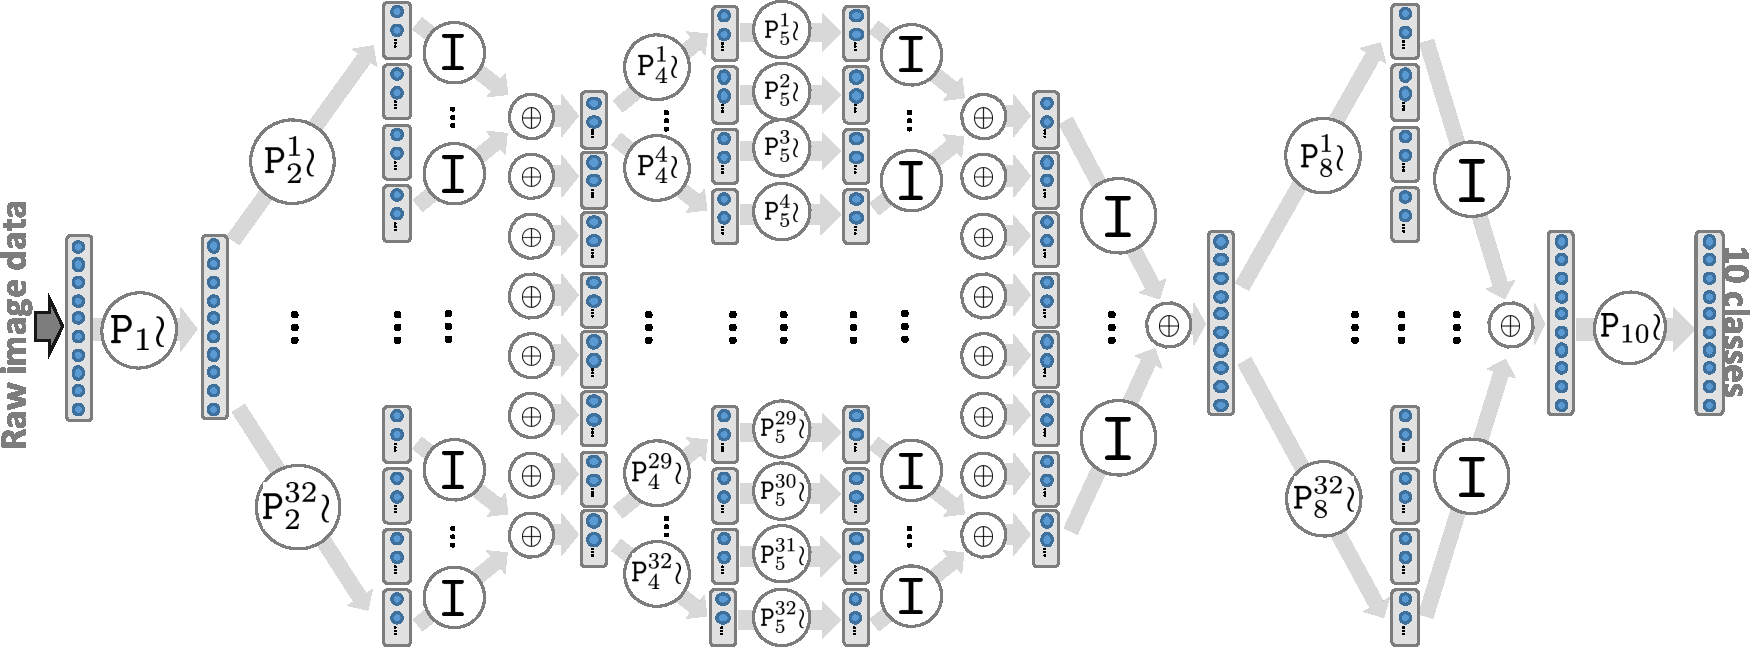
\includegraphics[width=0.98\linewidth]{resultsCifar_conditionalNetwork}
		}
		\caption[Automatically-learned conditional architecture for \Glsfmttext{cifar10}]{\textbf{Automatically learned conditional architecture for image classification in \Glsfmttext{cifar10}.} Both structure and parameters of this conditional network have been learned automatically via Bayesian optimization. \copyright Antonio Criminisi, used with permission.}
		\label{fig:Cifar_CondNet}
	\end{figure}
	
	\subsubsection{Designing a Family of Conditional Networks}
	The NiN model has a large number (192) of initial image-level filters in the first convolutional layer (`conv1'), 
	representing a sizable amount of the overall computation.\footnote{Most Imagenet networks typically use $64-96$ conv1 filters.}
	We build a variant (`NiN-64') that prepends a layer of 64 filters to the NiN model.
	While this variant is more complex than NiN, when routed (as described later) it allows us 
	to split the larger layers into many routes and increase the efficiency.
	In fact, for a convolutional layer with $N$ groups of filters, each filter operates on $1/N$ channels of the input \gls{featuremap}\index{feature map}, thus yielding reduced test-time computation and learning filters with fewer channels. 
	Additionally, training routed convolutional layers means that filters are exposed only to the training subset of data that flows through that route, thus allowing for a potentially higher degree of specialization.
	By changing the number of routes at each level of the NiN-64 model (from \texttt{conv2}) we can 
	generate a whole family of possible conditional architectures. 
	
	\subsubsection{Learning the Optimal Network Architecture}
	In this experiment we have optimized the network structure {\em automatically}, 
	by using Bayesian optimization~\citep{Snoek2012}, as available in WhetLab.\footnote{Formerly at \href{https://www.whetlab.com}{https://www.whetlab.com}, defunct since its \href{https://techcrunch.com/2015/06/17/twitter-acquires-machine-learning-startup-whetlab/}{acquisition by Twitter in June 2015}.} 
	This has allowed us to search the large joint space of parameters and structures in a principled manner, 
	and come up with multiple reasonable networks to be tested. 
	%\acnote{we have not done this in Imagenet because too big.}
	
	In the optimization we maximized the {\em size-normalized} accuracy $\alpha =\frac{\textrm{validation accuracy}}{\textrm{model size}}$ with respect to the parameters $R_l = 2^i, \left\{i\in \mathbb{N} : 0 \le i \le 5\right\}$, where $R_l$ is the number of nodes at layer $l$ in the conditional network. 
	\Cref{fig:Cifar_CondNet} shows the architecture which maximizes $\alpha$ in \gls{cifar10}. 
	It is a DAG-structured conditional network with 10 layers.
	To our knowledge this is the first attempt at learning automatically the architecture of a deep \gls{cnn} for image classification.
	
	\subsubsection{Accuracy \vs efficiency}
	For comparison, we also reduce the complexity of the unrouted NiN-64 network by learning a reduction in the number of per-layer filters, \ie we maximize $\alpha$ over $F_l = F_\textrm{orig}/2^i, \left\{i\in \mathbb{N} : 0 \le i \le 4\right\}$, where $F_\textrm{orig}$ is the number of filters in layer $l$ in NiN-64. 
	
	All networks were trained with the same hyperparameters as~\citep{Lin2013NiN}, 
	except for using the initialization strategy of~\citep{He2015b}, and a learning schedule,
    \begin{equation}
        \gls{lr}_t = \gls{lr}_0(1+\gls{lr}_0\gls{weightdecay} \gls{t})^{-1},
    \end{equation}
    where $\gls{lr}_0,\gls{lr}_t$ and $\gls{weightdecay}$ are the initial learning rate, learning rate at iteration $\gls{t}$, and weight decay\index{weight decay} respectively~\citep{Bottou2012sgdtricks}. Training was run for a maximum of 400 epochs, or until the maximum validation accuracy had not changed in 10,000 iterations. 
	We split the original \gls{cifar10} training set into 40,000 training images and 
	10,000 validation images. 
	The standard 10,000 held-out images are used for testing.
	
	\begin{figure}[tbp] 
		\centering
		\begin{subfigure}[b]{0.9\linewidth}
			\centering
			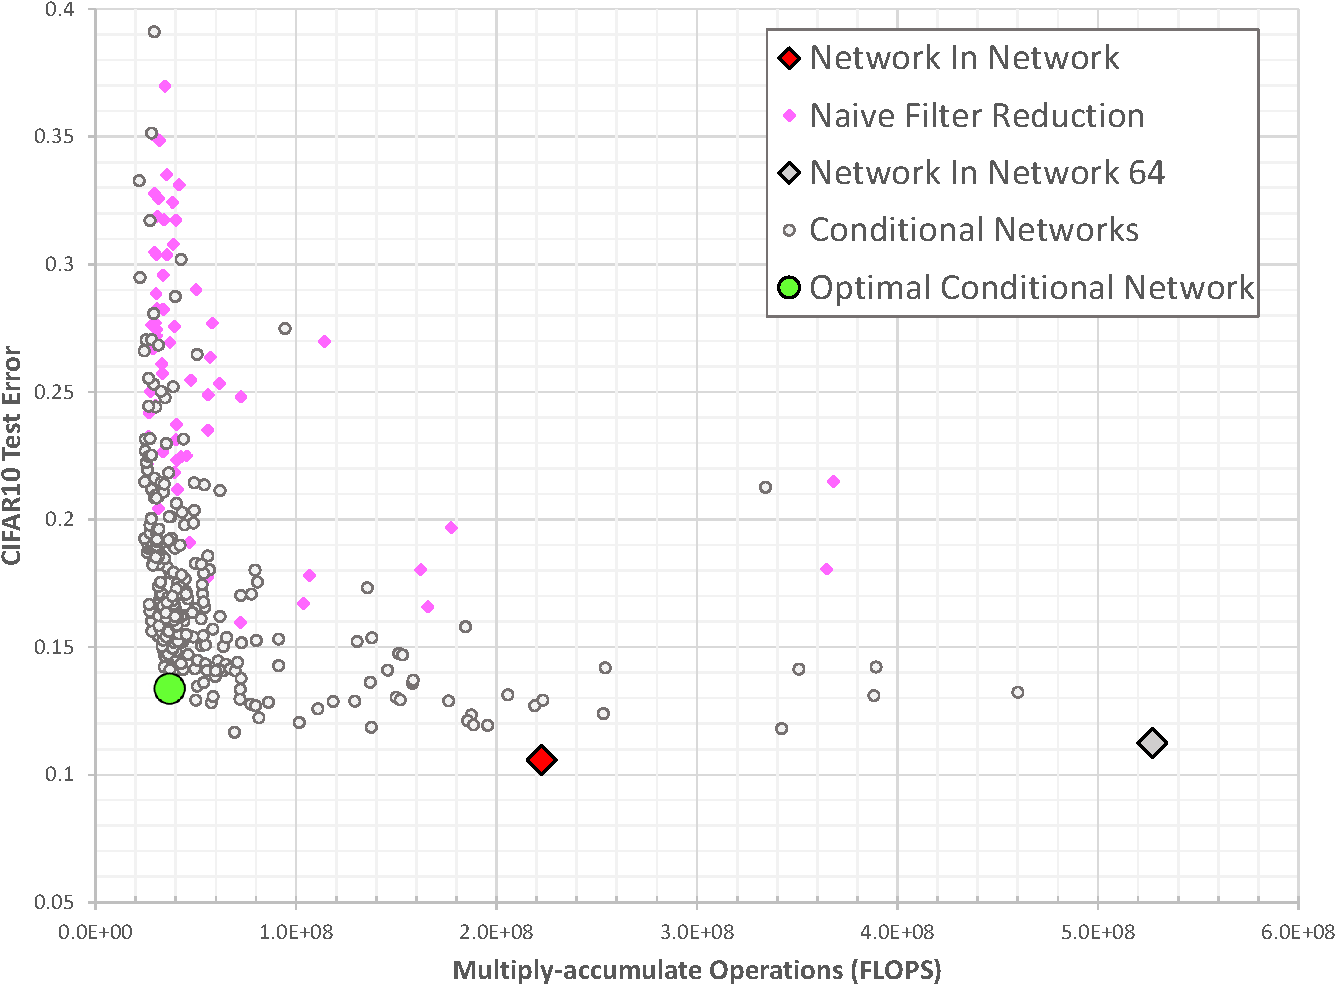
\includegraphics[width=\linewidth]{resultsCifar_AccVsEff}
			\caption{Test error \vs test-time computation for various architectures used in the CIFAR experiments.}\label{fig:resultsCifar_AccVsEff}
		\end{subfigure}
		~
		\begin{subfigure}[b]{0.9\linewidth}
			\centering
			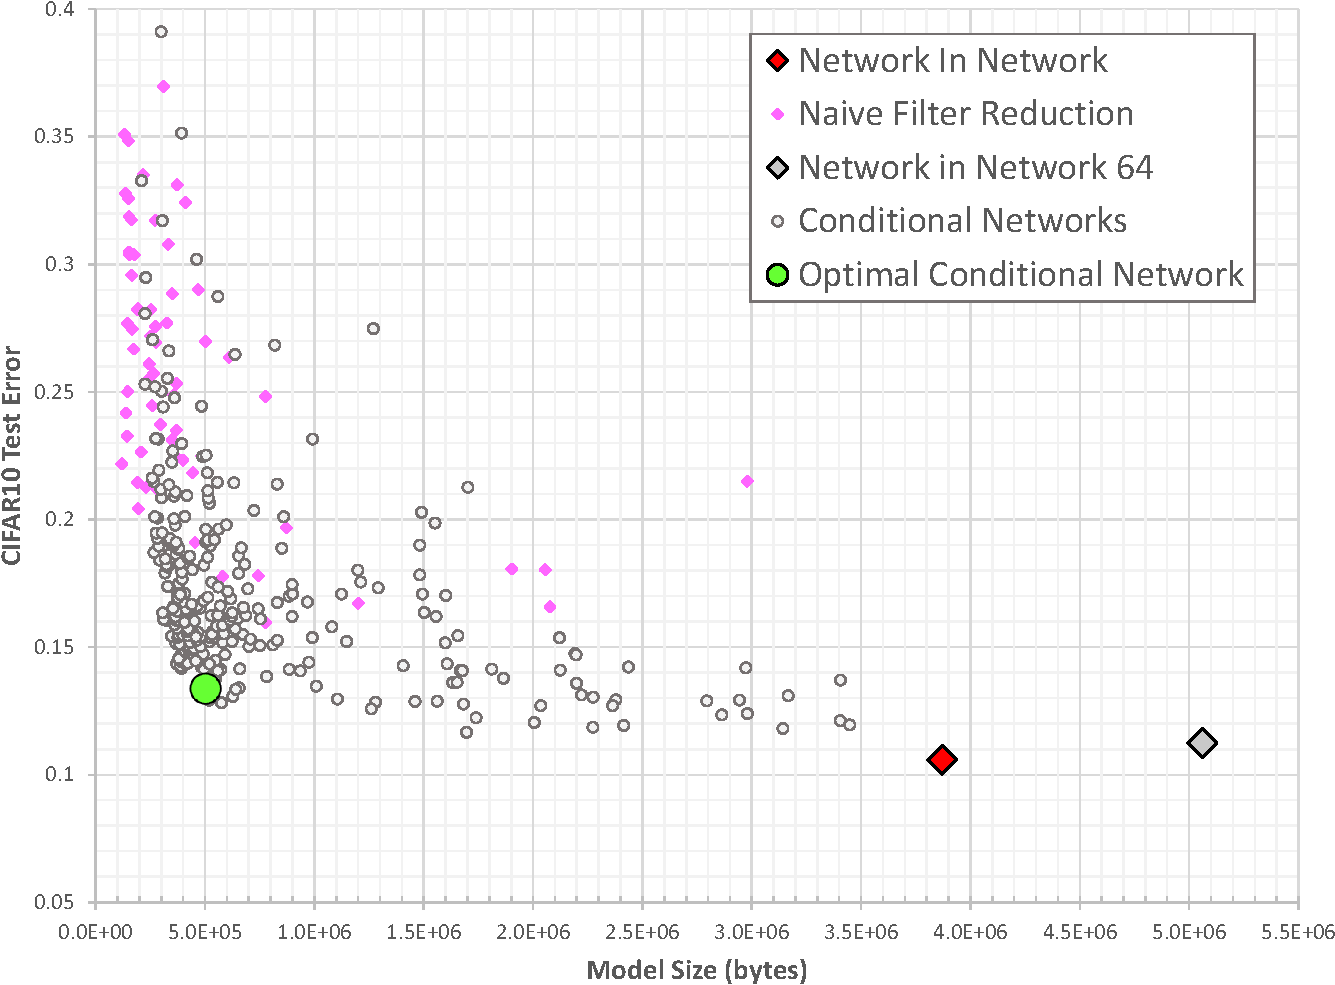
\includegraphics[width=\linewidth]{resultsCifar_AccVsSize}
			\caption{Test error \vs model size.}\label{fig:resultsCifar_AccVsSize}
		\end{subfigure}
		\caption[Comparing network architectures on \Glsfmttext{cifar10}]{\textbf{Comparing network architectures on \glsfmttext{cifar10}.} Conditional networks (denoted with circles) yield the points closest to the origin, corresponding to the best accuracy-efficiency trade-off. Our best conditional network is denoted with a green circle.}\label{fig:Cifar_results}
	\end{figure}
	%
	\Cref{fig:Cifar_results} shows test errors with respect to test-time cost and model size for multiple networks.
	Diamonds denote unrouted networks and circles denote conditional networks. 
	The original NiN is shown in red, and our NiN-64 variant is shown as a grey diamond.
	A sample of 300 models explored during the Bayesian optimization are shown as grey circles.
	The green circle denotes the conditional network closest to the origin of the 
	3D space $(\textrm{test-error}, \textrm{test-cost}, \textrm{model-size})$.
	Most of the conditional networks proposed by the Bayesian search procedure are distributed along a curve characterized by either high accuracy, or low model size, or both. 
	Reducing the NiN model by filter reduction (pink diamonds in the figure) does not yield the same gains as data routing.
	Despite NiN achieving the highest accuracy (it has been optimized for accuracy alone), the optimal conditional network is much closer to the origin of the 3D space, thus indicating much higher efficiency (in terms of memory and computation) for a small loss in accuracy.
	
	\section{Discussion}

%\vspace{-0.5\baselineskip}

This chapter has investigated the similarities and differences between decision trees/forests and \gls{dnn}. This has led us to introduce a hybrid model (namely conditional networks) which can be thought both as: 
\begin{enumerate*}[label= (\textbf{\roman*})]
\item trees which have been augmented with representation learning capabilities, and
\item \glspl{cnn}\index{CNN} which have been augmented with explicit data routers and a rich, branched architecture.
\end{enumerate*}
Experiments on image classification have shown that highly branched architectures yield improved accuracy-efficiency trade-off as compared to trees or \glspl{cnn}\index{CNN}. The desired accuracy-efficiency ratio can be selected \emph{at run time}, without the need to train a new network.
%Finally, we have shown how explicit routers can improve the efficiency of {\em ensembles} of \glspl{cnn}\index{CNN}, without loss of accuracy.
	
\end{document}
